\chapter{Results}\label{ch:results}

This chapter presents the experimental results of different DIP-based denoising approaches.
We first evaluate these methods on standard image datasets, providing a controlled setting for method comparison.
Then, we apply these approaches to DAS data demonstrating its performance in a more complex real-world scenario.

\section{Image Data}

Since clean reference samples are not available for DAS data, we begin by conducting experiments on standard image denoising tasks.
These preliminary evaluations enable a controlled comparison of different methods and configurations.

For all variants, we follow the original DIP paper and set the maximum number of iterations to 2000.
For ES-based methods, we employ the ES-WMV criterion with a patience of 500 iterations.
For DIP-TV, we set $\lambda = 0.1$, and for SG-DIP, we set the number of different noise samples per iteration to 3, as recommended in the original paper.

As discussed in Section~\ref{sec:architecture}, we use ECA in the skip connections because it tends to retain more fine-grained details, while yielding almost identical performance, as shown in Table~\ref{tab:ECA}. 

\begin{table}
    \centering
    \begin{tabular}{ l l c c }
        \toprule
        Skip Type &Method &PSNR (dB) $\uparrow$ &SSIM $\in [0,1]$ $\uparrow$ \\
        \midrule
        \multirow{2}{4em}{Conv} &SG-DIP (ES) &26.03 {\scriptsize (2.15)} &0.68 {\scriptsize (0.11)} \\
        &SGR-DIP &\underline{26.34} {\scriptsize (2.12)} &\textbf{0.70} {\scriptsize (0.11)} \\
        \midrule
        \multirow{2}{4em}{ECA} &SG-DIP (ES) &25.97 {\scriptsize (1.92)} &0.68 {\scriptsize (0.11)} \\
        &SGR-DIP &\textbf{26.37} {\scriptsize (2.04)} &\textbf{0.70} {\scriptsize (0.11)} \\
        \bottomrule
    \end{tabular}
    \caption{
        Comparison of different types of skip connections on the Set14 dataset.
        Noisy input images are generated at a PSNR of 10\,dB.
        Values represent mean and {\scriptsize (standard deviation)}.
    }\label{tab:ECA}
\end{table}

\begin{figure}
    \centering
    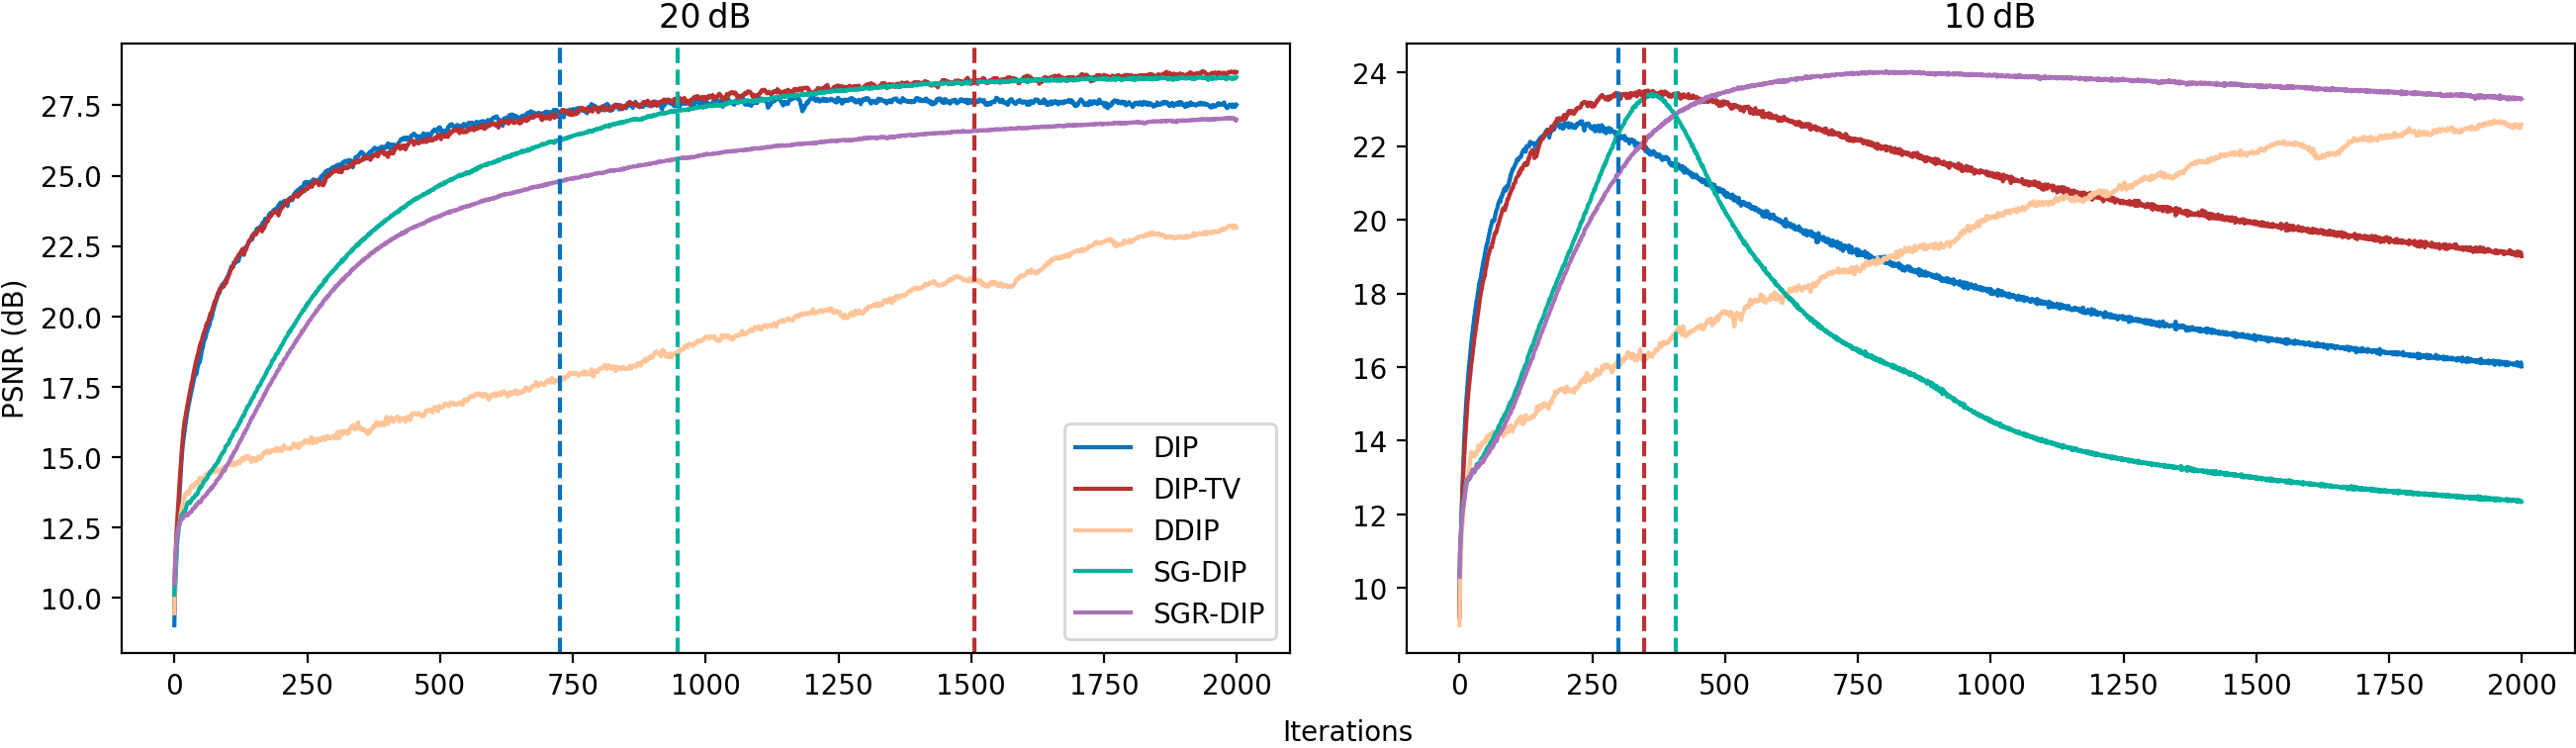
\includegraphics[width=0.875\textwidth]{img/fig_6.1.png}
    \caption{
        Visual comparison of different DIP variants on the CBSD68 dataset.
        Noisy input images are generated at a PSNR of 15\,dB.
    }\label{fig:CBSD68}
\end{figure}

\begin{table}
    \centering
    \begin{tabular}{ l c c c }
        \toprule
        Method &PSNR (dB) $\uparrow$ &SSIM $\in [0,1]$ $\uparrow$ &Runtime (m) $\downarrow$\\
        \midrule
        DIP &22.32 {\scriptsize (0.74)} &0.43 {\scriptsize (0.11)} &\underline{1.31} {\scriptsize (0.01)} \\
        DIP (ES) &25.64 {\scriptsize (2.07)} &0.62 {\scriptsize (0.07)} &\textbf{0.50} {\scriptsize (0.08)} \\
        DIP-TV &26.06 {\scriptsize (1.37)} &0.65 {\scriptsize (0.07)} &1.45 {\scriptsize (0.01)} \\
        DDIP &24.54 {\scriptsize (3.15)} &0.61 {\scriptsize (0.13)} &1.34 {\scriptsize (0.01)} \\
        SG-DIP (ES) &\underline{26.57} {\scriptsize (2.47)} &\underline{0.69} {\scriptsize (0.09)} & 2.05 {\scriptsize (0.61)} \\
        SGR-DIP &\textbf{26.76} {\scriptsize (2.51)} &\textbf{0.70} {\scriptsize (0.10)} & 3.34 {\scriptsize (0.09)} \\
        \bottomrule
    \end{tabular}
    \caption{
        Quantitative comparison of different DIP variants on the CBSD68 dataset.
        Noisy input images are generated at a PSNR of 15\,dB.
        Values represent mean and {\scriptsize (standard deviation)}.
    }\label{tab:CBSD68}
\end{table}

Table~\ref{tab:CBSD68} presents the performance of the different DIP variants discussed in this work in terms of PSNR and SSIM\@.
Corresponding visual comparisons between the methods are available in~\ref{fig:CBSD68}.
Our method yields the best results; however, it is significantly slower than other approaches.

% TODO 10 dB vs 20 dB - table & PSNR/SSIM curves

\section{Distributed Acoustic Sensing Data}
